\documentclass{article}
\usepackage{amsmath,amssymb,amsthm}
\usepackage{listings}
\usepackage{graphicx}
\usepackage[shortlabels]{enumitem}
\usepackage{tikz}
\usepackage[margin=1in]{geometry}
\usepackage{fancyhdr}
\usepackage{epsfig} %% for loading postscript figures
\usepackage{amsmath}
\usepackage{float}
\usepackage{amssymb}
\usepackage{caption}
\usepackage{subfigure}
\usepackage{graphics}
\usepackage{titlesec}
\usepackage{mathrsfs}
\usepackage{amsfonts}
\usepackage{indentfirst}
\usepackage{color}

\renewcommand{\baselinestretch}{1.2}%Adjust Line Spacing
%\geometry{left=2.0cm,right=2.0cm,top=2.0cm,bottom=2.0cm}% Adjust Margins of the File
\usepackage{tikz-qtree}
\usetikzlibrary{graphs}
\tikzset{every tree node/.style={minimum width=2em,draw,circle},
	blank/.style={draw=none},
	edge from parent/.style=
	{draw,edge from parent path={(\tikzparentnode) -- (\tikzchildnode)}},
	level distance=1.2cm}
\setlength{\parindent}{0pt}
%\setlength{\parskip}{5pt plus 1pt}
\setlength{\headheight}{13.6pt}
\newcommand\question[2]{\vspace{.25in}\hrule\textbf{#1: #2}\vspace{.5em}\hrule\vspace{.10in}}
\renewcommand\part[1]{\vspace{.10in}\textbf{(#1)}}
\newcommand\algorithm{\vspace{.10in}\textbf{Algorithm: }}
\newcommand\correctness{\vspace{.10in}\textbf{Correctness: }}
\newcommand\runtime{\vspace{.10in}\textbf{Running time: }}
\pagestyle{fancyplain}
% Create horizontal rule command with an argument of height
\newcommand{\horrule}[1]{\rule{\linewidth}{#1}}



% Set the title here
\title{
	\normalfont \normalsize
	\textsc{ShanghaiTech University} \\ [25pt]
	\horrule{0.5pt} \\[0.4cm] % Thin top horizontal rule
	\huge CS101 Algorithms and Data Structures\\ % The assignment title
	\LARGE Fall 2021\\
	\LARGE Homework 12\\
	\horrule{2pt} \\[0.5cm] % Thick bottom horizontal rule
}
% wrong usage of \author, never mind
\author{}
\date{Due date: 23:59, January 3, 2022}

% set the header and footer
\pagestyle{fancy}
\lhead{CS101 Algorithms and Data Structures}
\chead{Homework 12}
\rhead{Due date: 23:59, January 3, 2022}
\cfoot{\thepage}
\renewcommand{\headrulewidth}{0.4pt}
\newtheorem{Q}{Question}
% special settings for the first page
\fancypagestyle{firstpage}
{
	\renewcommand{\headrulewidth}{0pt}
	\fancyhf{}
	\fancyfoot[C]{\thepage}
}

% Add the support for auto numbering
% use \problem{title} or \problem[number]{title} to add a new problem
% also \subproblem is supported, just use it like \subsection
\newcounter{ProblemCounter}
\newcounter{oldvalue}
\newcommand{\problem}[2][-1]{
	\setcounter{oldvalue}{\value{secnumdepth}}
	\setcounter{secnumdepth}{0}
	\ifnum#1>-1
	\setcounter{ProblemCounter}{0}
	\else
	\stepcounter{ProblemCounter}
	\fi
	\section{Problem \arabic{ProblemCounter}: #2}
	\setcounter{secnumdepth}{\value{oldvalue}}
}
\newcommand{\subproblem}[1]{
	\setcounter{oldvalue}{\value{section}}
	\setcounter{section}{\value{ProblemCounter}}
	\subsection{#1}
	\setcounter{section}{\value{oldvalue}}
}

% \setmonofont{Consolas}
\definecolor{blve}{rgb}{0.3372549 , 0.61176471, 0.83921569}
\definecolor{gr33n}{rgb}{0.29019608, 0.7372549 , 0.64705882}
\makeatletter
\lst@InstallKeywords k{class}{classstyle}\slshape{classstyle}{}ld
\makeatother
\lstset{language=C++,
	basicstyle=\ttfamily,
	keywordstyle=\color{blve}\ttfamily,
	stringstyle=\color{red}\ttfamily,
	commentstyle=\color{magenta}\ttfamily,
	morecomment=[l][\color{magenta}]{\#},
	classstyle = \bfseries\color{gr33n}, 
	tabsize=4
}
\lstset{basicstyle=\ttfamily}
\begin{document}

\maketitle
\thispagestyle{firstpage}
%\newpage
\vspace{3ex}

\begin{enumerate}
	\item Please write your solutions in English.

	\item Submit your solutions to gradescope.com.

	\item Set your FULL NAME to your Chinese name and your STUDENT ID correctly in Account Settings.

	\item If you want to submit a handwritten version, scan it clearly. Camscanner is recommended.

	\item When submitting, match your solutions to the according problem numbers correctly.

	\item No late submission will be accepted.

	\item Violations to any of the above may result in zero grade.

	\item {\large\color{red}{In this homework, all the proofs need three steps. The demands and an example are given on the next page. If you do not organize your answer in the standard format, you will not get any point.}}
\end{enumerate}
\newpage
\section*{Demand of the NP-complete Proof}
When proving problem A is NP-complete, please clearly divide your answer into three steps:
\begin{enumerate}

	\item Prove that problem A is in NP.

	\item Choose an NP-complete problem B and for any B instance, construct an instance of problem A.

	\item Prove that the yes/no answers to the two instances are the same.
\end{enumerate}
\section*{Proof Example}
Suppose you are going to schedule courses for the SIST and try to make the number of conflicts no more than K. You are given 3 sets of inputs: $C=\{\cdots\},S=\{\cdots\},R=\{\{\cdots\},\{\cdots\},\cdots\}$. C is the set of distinct courses. S is the set of available time slots for all the courses. R is the set of requests from students, consisting of a number of subsets, each of which specifies the course a student wants to take. A conflict occurs when two courses are scheduled at the same slot even though a student requests both of them. Prove this schedule problem is NP-complete.\\
\textcolor{blue}{
	\begin{enumerate}
		\item Firstly, for any given schedule as a certificate, we can traverse every student's requests and check whether the courses in his/her requests conflicts and count the number of conflicts, and at last check if the total number is fewer than K, which can be done in polynomial time. Thus the given problem is in NP.
		\item We choose 3-coloring problem which is a NP-complete problem. For any instance of 3-coloring problem with graph $G$, we can construct an instance of the given problem: let every node $v$ becomes a course, thus construct $C$; let every edge $(u,v)$ becomes a student whose requests is $\{u,v\}$, thus construct $R$; let each color we use becomes a slot, thus construct $S$; at last let $K$ equals to $0$.
		\item We now prove $G$ is a yes-instance of 3-coloring problem if and only if $(C,S,R,K)$ is a yes-instance of
		      the given problem:
		      \begin{itemize}
			      \item "$\Rightarrow$": if $G$ is a yes-instance of 3-coloring problem, then schedule the courses according to their color. Since for each edge $(u,v)$, $u$ and $v$ will be painted with different color, then for each student, his/her requests will not be scheduled to the same slot, which means the given problem is also a yes-instance.
			      \item "$\Leftarrow$": if $(C,S,R,K)$ is a yes-instance of the given problem, then painting the nodes in $G$ according to their slots. Since $K=0$, then for every student, there is no conflict between their requests, which suggests that for every edge $(u,v)$, $u$ and $v$ will not be painted with the same color. It is also a yes-instance of 3-coloring problem.
		      \end{itemize}
	\end{enumerate}
	Therefore, the given problem is NP-complete.
}
\newpage

\question{1}{(3'+3'+4') Multiple Choice}
The following \textit{} questions are multiple choice questions, each question may have one or more correct answers. Select all correct answers.\\
\textit{Note: You should write those answers \textbf{in the box} below.}

\begin{table}[htbp]
	\begin{tabular}{|p{2cm}|p{2cm}|p{2cm}|}
		\hline
		Question 1 & Question 2 & Question 3 \\
		\hline
		B          & D          & BC         \\
		\hline
	\end{tabular}
\end{table}



\begin{Q}
	A problem in NP is NP-complete if:
	\begin{enumerate}[(A)]
		\item It can be reduced to the 3-SAT problem in polynomial time.
		\item The 3-SAT problem can be reduced to it in polynomial time.
		\item It can be reduced to any other problem in NP in polynomial time.
		\item Some problem in NP can be reduced to it in polynomial time.
	\end{enumerate}
\end{Q}


\begin{Q}
	Suppose we have found an algorithm which correctly solves the vertex cover problem in polynomial time. Then under this circumstance, which one of the following Venn diagrams correctly represents the relationship among the complexity classes P, NP and NP Complete (NPC)?
	\begin{center}
		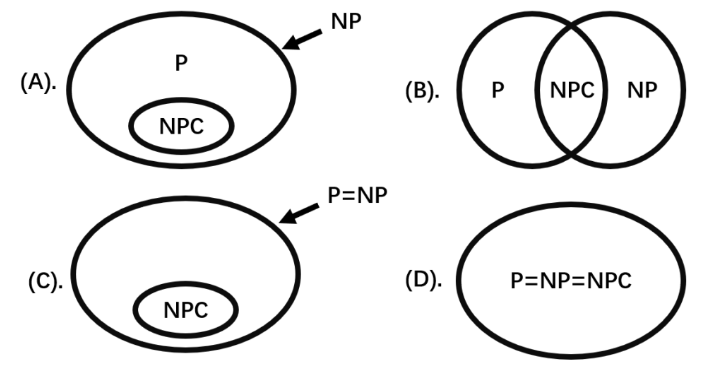
\includegraphics[scale=0.7]{HW12-Q2.png}
	\end{center}
\end{Q}

\begin{Q}
	Assume problem A reduces to problem B in polynomial time. Which of the following choice(s) is/are correct?
	\begin{enumerate}[(A)]
		\item If A is in \textbf{P}. Then B is in \textbf{P}.
		\item If B is in \textbf{P}. Then A is in \textbf{P}.
		\item If A is \textbf{NP}-hard. Then B is \textbf{NP}-hard.
		\item If B is \textbf{NP}-hard. Then A is \textbf{NP}-hard.
	\end{enumerate}
\end{Q}

\pagebreak
%%%%%%%%%%%%%%%%%%%%%%%%%%%%%
\question{2}{(10') 4-COLOR}
Given an undirected graph and 4 different colors, can we color the nodes so that no adjacent nodes have the same color? Show that the 4-COLOR problem is NP-complete. \textbf{(Hint: Reduce from 3-COLOR)}

\textcolor{blue}{
	\begin{enumerate}
		\item Firstly, for any given colored graph $G(V,E)$ as a certificate, we can traverse all the egdes $(u,v)\in E$ to see if there exists any egde that both vertices linked by it are in the same color. If there is no such edge, then the graph $G$ is a yes-instance. The certifier can be conducted in polynomial time, thus the problem is in NP.
		\item We choose 3-coloring problem to reduce from which is a NP-complete problem. Given a 3-color instance $G$, we construct an instance of 4-color that is 4-colorable iff $G$ is 3-colorable. We can create a vertex that is connected to every vertices in the 3-coloring instance $G$.
		\item Now prove for such instance constructed, it is 4-colorable iff G is 3-colorable:
		      \begin{itemize}
			      \item "$\Rightarrow$": if $G$ is a yes-instance of 3-coloring problem, then we can just color the newly added vertex with a new color (the forth color), thus making it a yes-instance for 4-coloring.
			      \item "$\Leftarrow$": if $G_1$ is a yes-instance of such constructed 4-coloring, as the newly add vertex is connected to all vertices in the original graph, it is in a unique color, the the total number of color of the rest of the graph (namely the original graph) is 3, proving the original graph is a yes-instance of 3-coloring.
		      \end{itemize}
	\end{enumerate}
	Therefore, the given problem is NP-complete.
}
\pagebreak

% ======================================

\question{3}{(10') Reduction from Independent Set}
Given a set $E$ and $m$ subsets of $E, S_1, S_2,..., S_m$, is there a way to select $k$ of the $m$ subsets such that the selected subsets are pairwise disjoint?

Show that this problem is NP complete. \\
HINT: Reduction from Independent Set.

\textcolor{blue}{
	\begin{enumerate}
		\item Firstly, for any given k subsets as a certificate, we can traverse all elements in the k subsets to see if there is any element that appears more than once. If there is none, then the certificate is a yes-instance for the problem. The certifier can be conducted in polynomial time, so the problem is in NP.
		\item We choose Independent Set to reduce from. Given an Independent Set instance $G=(V,E)$ and k, we construct an instance for this problem that have k pairwise disjoint subsets iff G has a independent set of size k: create m subsets, corresponding to the m($=|V|$) vertices in the independent set problem, mark all edges in G in order, then let each of the m subsets contains all edges that it is incident to (as numbers). Then prove the following lemma: $G=(V,E)$ contains a independent set of size k iff there are k subsets constructed like this are pairwise disjoint.
		\item \begin{itemize}
			      \item "$\Rightarrow$": if a instance is a independent set of size k, then just select the k subsets mapped from the k vertices. The k subsets has no common element, since the k vertices don't share any edge.
			      \item "$\Leftarrow$": if a instance is k subsets that are pairwise disjoint, then the k vertices mapped from the k subsets share no egde, thus making it a independent set of size k.
		      \end{itemize}
	\end{enumerate}
	Therefore, the given problem is NP-complete.
}

\pagebreak
% =========================
\question{4}{(10') Exact 4-SAT problem}

In the Exact 4-SAT problem, the input is a set of clauses, each of which is a disjunction of exactly four literals, and such that each variable occurs at most once in each clause. The goal is to find a satisfying argument, if one exists. Prove that Exact 4-SAT is NP-complete by a reduction from 3-SAT.

\textcolor{blue}{
	\begin{enumerate}
		\item Firstly, for any given CNF and the boolean value of each variable as a certificate, we can pluge these value into all literals to get the boolean value of the CNF, which takes polynomial time, so the given problem is in NP.
		\item We choose 3-SAT to reduce from. Given an instance of 3-SAT, we construct an instance of 4-SAT: replace every clause in 3-SAT with two clauses, each of them contains one literal more, itself and its negation respectively. For example, the clause $(x_1\vee x_2\vee x_3)$ is transformed to $(x_1\vee x_2\vee x_3\vee y)\wedge (x_1\vee x_2\vee x_3\vee \bar{y})$. Then we have to prove that a 3-sat CNF is satisfiable iff such constructed 4-sat CNF is satisfiable.
		\item \begin{itemize}
			\item "$\Rightarrow$": If a CNF is 3-satisfiable, for each of its clause, for example $(x_1\vee x_2\vee x_3)$, returns true, thus making both $(x_1\vee x_2\vee x_3\vee y)$ and $(x_1\vee x_2\vee x_3\vee \bar{y})$ return true.
			\item "$\Leftarrow$": If a CNF of 4-sat constructed in this way is satisfiable, then we pay attention to segmentations of it, for example $(x_1\vee x_2\vee x_3\vee y)\wedge (x_1\vee x_2\vee x_3\vee \bar{y})$, both of the clauses return true. Then we can find that if $y$ is true, then $(x_1\vee x_2\vee x_3)$ must be true since $(x_1\vee x_2\vee x_3\vee \bar{y})$ is true; and if $y$ is false, still $(x_1\vee x_2\vee x_3)$ must be true since $(x_1\vee x_2\vee x_3\vee y)$ is true. Thus ensuring such e-sat is also satisfiable.
		\end{itemize}
		Therefore, the given problem is NP-complete.
	\end{enumerate}
}

\end{document}